\chapter{生态系统与营养结构}\label{ch:b1:ecosystem-organization}

石灰岩平原上的一眼泉水清澈见底，
从船上就能数清其中的每一株植物、每一条鱼和每一只龟。
落在眼子菜上的阳光为每平方米每年 170 万千卡；
这种草储存其中的百分之一；
吃草的螺和龟获得其中的六分之一；
吃螺的鱼再获得十分之一；
处于顶端的那只苍鹭，所得仅为落在水面上能量的十万分之一。
每个\omterm{def:b1:ecosystem-organization:ecosystem}{生态系统}都是这样构成的：能量流入一次，从食者流向被食者，
最终以热量散失，而它所携带的物质则被循环利用。
本章定义\omterm{def:b1:ecosystem-organization:ecosystem}{生态系统}及其组成部分，每个物种所占据的\omterm{def:b1:ecosystem-organization:niche}{生态位}，
能量流经的\omterm{def:b1:ecosystem-organization:trophic}{营养级}与\omterm{def:b1:ecosystem-organization:foodweb}{食物网}，
决定整个系统规模的生产力，以及
统计其中生物种类数的方法。

\section{生态系统与生态位}

\begin{definition}[生态系统、生境、群落]\label{def:b1:ecosystem-organization:ecosystem}
\index{生态系统}\index{生境}\index{群落}
\emph{生态系统}是指在一定区域内生活的\omterm{def:b1:organism-environment:organism}{生物体}，
连同它们所占据并与之交换物质和能量的物理\omterm{def:b1:organism-environment:organism}{环境}所组成的整体：
\emph{群落}（或称生物群落）——即所有物种的全部\omterm{def:b1:populations:population}{种群}——
以及\emph{生境}——即土壤、水、空气、光照和气候。
其边界根据所研究的问题而定：一段腐烂的原木、一个池塘、
一片森林、一个海盆，乃至整个生物圈，都可以作为生态系统。
生态系统是一个开放系统（见\cref{ch:b1:organism-environment}）：
能量单向流经它，物质则在其内部及其边界之间循环，
其结构即为谁吃谁的模式。
\end{definition}

\begin{definition}[栖息地、生态位]\label{def:b1:ecosystem-organization:niche}
\index{生态位}\index{栖息地}
物种的\emph{栖息地}是它所生活的场所；其\emph{生态位}则是它的生活方式：
即它所耐受的全部条件与所利用的全部资源——
温度、湿度、光照、食物、活动时间、筑巢地点——
其中每一项都是一个维度，物种在各维度上占据
一定范围。\emph{基础生态位}是指该物种单独存在时可能占据的范围；
\emph{实际生态位}则是在竞争者和捕食者存在时它实际占据的部分
（见\cref{ch:b1:species-interactions}）。
生态位相同的两个物种难以长期共存于同一地点；
共存物种的生态位各不相同，\omterm{def:b1:ecosystem-organization:ecosystem}{群落}正是
由相互契合的生态位组成的。
\end{definition}

\begin{omfigure}
\begin{tikzpicture}[font=\footnotesize, >=Stealth, line cap=round]
  \draw[->, thick] (0,0) -- (7.4,0) node[below left] {温度};
  \draw[->, thick] (0,0) -- (0,5.2) node[below right, rotate=90, anchor=south east] {};
  \node[rotate=90, anchor=south] at (-0.4,2.6) {猎物大小};
  \draw[thick, omDef, fill=omDef!18] (3.6,2.6) ellipse (2.8 and 1.9);
  \node[omDef!80!black, anchor=south] at (2.5,3.7) {基础生态位};
  \draw[thick, omThm, fill=omThm!25] (2.9,2.3) ellipse (1.6 and 1.2);
  \node[omThm!80!black] at (2.9,2.3) {实际生态位};
  \draw[thick, omProp, fill=omProp!25, opacity=0.8] (5.6,3.4) ellipse (1.5 and 1.1);
  \node[omProp!80!black, align=center] at (5.6,3.4) {竞争者的 \\ 生态位};
  \node[anchor=north, align=center, gray] at (3.7,-0.5) {生态位众多维度中的两个；竞争者将该物种排挤出重叠部分};
\end{tikzpicture}

{\small \omterm{def:b1:ecosystem-organization:niche}{生态位}是条件与资源构成的空间中的一个体积，
图中画出了其中两个维度。基础\omterm{def:b1:ecosystem-organization:niche}{生态位}是物种可能占据的范围；
实际\omterm{def:b1:ecosystem-organization:niche}{生态位}则是其竞争者
留给它的部分。}
\end{omfigure}

\begin{example}[同一云杉上的五种莺]\label{ex:b1:ecosystem-organization:warblers}
五种食虫的小型莺都在同一片云杉林中筑巢，
取食相同的昆虫；仔细观察便会发现，每个物种觅食的部位各不相同——
树梢、外侧的新针叶、中部枝条、
树干和下部枝条、树下地面——而且觅食的高度和时间也不同。
它们的\omterm{def:b1:ecosystem-organization:niche}{栖息地}是同一个，
而\omterm{def:b1:ecosystem-organization:niche}{生态位}却有五个；按食物推测只能有一个物种，
而森林中却养活着五个物种。
\end{example}

\section{营养结构}

\begin{definition}[生产者、消费者、分解者]\label{def:b1:ecosystem-organization:trophic}
\index{营养级}\index{生产者}\index{消费者}\index{分解者}
\omterm{def:b1:ecosystem-organization:ecosystem}{生态系统}中的生物按其食性划分为若干
\emph{营养级}。\emph{生产者}（\omterm{def:b1:photosynthesis:autotrophy}{自养}生物：植物、藻类、蓝细菌、化能合成细菌）
将无机物合成为有机物，是第一营养级。
\emph{消费者}以之为食：\emph{初级消费者}（植食性动物）取食生产者，
\emph{次级消费者}（肉食性动物）取食植食性动物，
\emph{三级}消费者取食肉食性动物；杂食性动物则在多个营养级上取食。
\emph{分解者}（细菌、真菌）
与\emph{食碎屑者}（蚯蚓、潮虫、粪甲虫）以死亡的有机体及各营养级的废物为生，
并将其中的矿物质归还土壤与水体，
供生产者再次吸收利用——
正是这一环节使物质的循环得以闭合。
\end{definition}

\begin{definition}[食物链、食物网]\label{def:b1:ecosystem-organization:foodweb}
\index{食物链}\index{食物网}
\emph{食物链}是由若干生物依次取食前一环节而构成的序列：
草、蝗虫、青蛙、蛇、鹰。在真实的\omterm{def:b1:ecosystem-organization:ecosystem}{群落}中，每个物种通常取食多种生物，
也被多种生物取食，各条食物链相互交织，
形成\emph{食物网}。食物网中的箭头由被食者指向取食者，
即能量流动的方向。食物链通常很短：
很少超过四到五个环节，
其原因将在下一节说明。
\end{definition}

\begin{omfigure}
\begin{tikzpicture}[font=\footnotesize, >=Stealth, line cap=round,
  sp/.style={draw, thick, rounded corners=3pt, inner sep=3pt, align=center, fill=white}]
  \node[sp, fill=omExo!20] (grass) at (1.5,0) {眼子菜、藻类};
  \node[sp, fill=omExo!20] (det) at (6.5,0) {碎屑};
  \node[sp, fill=omProp!20] (snail) at (0,2.0) {螺};
  \node[sp, fill=omProp!20] (insect) at (2.6,2.0) {昆虫幼虫};
  \node[sp, fill=omProp!20] (turtle) at (5.0,2.0) {龟};
  \node[sp, fill=omProp!20] (shrimp) at (7.6,2.0) {虾、蠕虫};
  \node[sp, fill=omThm!20] (sunfish) at (1.3,4.0) {翻车豚};
  \node[sp, fill=omThm!20] (catfish) at (6.4,4.0) {鲶鱼};
  \node[sp, fill=omDef!25] (bass) at (2.8,5.8) {鲈鱼};
  \node[sp, fill=omDef!25] (heron) at (6.0,5.8) {苍鹭};
  \node[sp, fill=gray!20] (dec) at (10.2,1.0) {细菌、真菌 \\ （分解者）};
  \draw[->, thick] (grass) -- (snail); \draw[->, thick] (grass) -- (insect); \draw[->, thick] (grass) -- (turtle);
  \draw[->, thick] (det) -- (shrimp); \draw[->, thick] (det) -- (insect);
  \draw[->, thick] (snail) -- (sunfish); \draw[->, thick] (insect) -- (sunfish); \draw[->, thick] (insect) -- (catfish); \draw[->, thick] (shrimp) -- (catfish);
  \draw[->, thick] (sunfish) -- (bass); \draw[->, thick] (sunfish) -- (heron); \draw[->, thick] (catfish) -- (heron); \draw[->, thick] (catfish) -- (bass);
  \draw[->, thick] (turtle) -- (heron);
  \draw[->, thick, gray, dashed] (9.0,0.4) -- (dec); \node[gray, font=\scriptsize, anchor=north] at (9.0,0.3) {所有死亡有机物};
  \node[anchor=east, omExo!70!black] at (-0.6,0) {生产者};
  \node[anchor=east, omProp!80!black] at (-0.6,2.0) {初级消费者};
  \node[anchor=east, omThm!80!black] at (-0.6,4.0) {次级消费者};
  \node[anchor=east, omDef!80!black] at (-0.6,5.8) {三级消费者};
\end{tikzpicture}

{\small 清澈泉水中的简化\omterm{def:b1:ecosystem-organization:foodweb}{食物网}。箭头自
食物指向取食者，方向即能量流动的方向；多数物种
在不止一个\omterm{def:b1:ecosystem-organization:trophic}{营养级}上取食，一切最终归于\omterm{def:b1:ecosystem-organization:trophic}{分解者}。}
\end{omfigure}

\begin{omfigure}
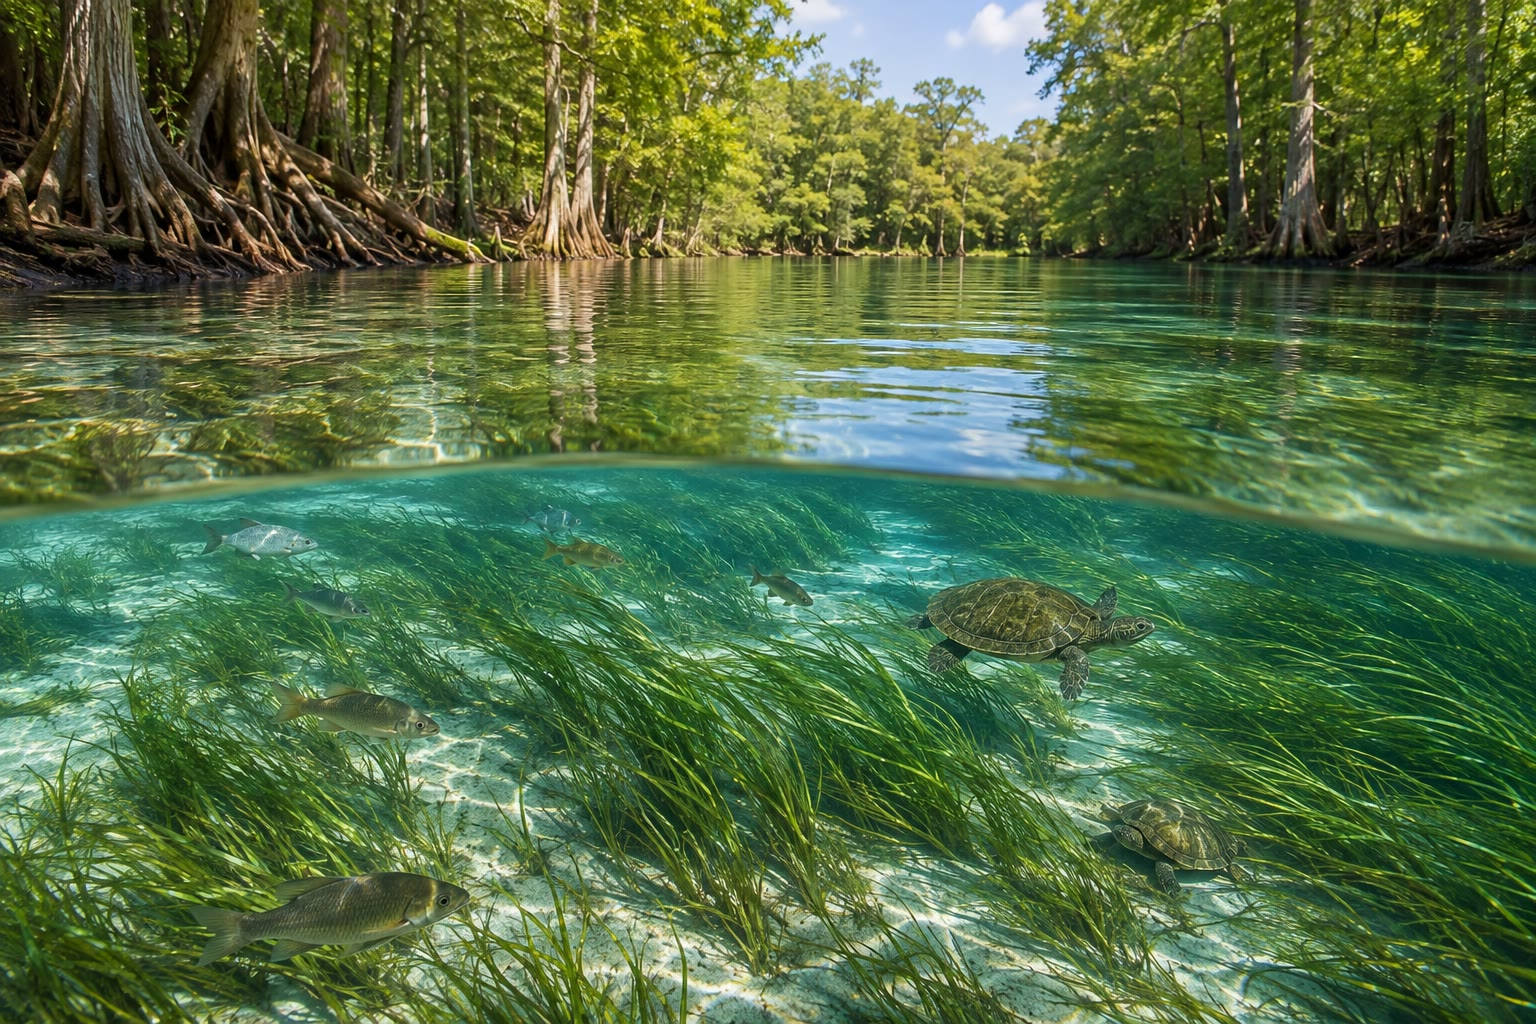
\includegraphics[width=0.6\linewidth]{images/book3/ai/b3-26-clear-spring.jpg}

{\small 石灰岩泉：\omterm{def:b1:ecosystem-organization:trophic}{生产者}层由大叶藻和藻类组成，
处于充足光照之下，其上为首份生态能量
收支所针对的\omterm{def:b1:ecosystem-organization:trophic}{消费者}。}
\end{omfigure}

\section{能量流动}

\begin{definition}[生产力]\label{def:b1:ecosystem-organization:productivity}
\index{初级生产力}\index{总初级生产力}\index{净初级生产力}
\omterm{def:b1:ecosystem-organization:ecosystem}{生态系统}的\emph{总初级生产力}（GPP）是指
\omterm{def:b1:ecosystem-organization:trophic}{生产者}通过光合作用固定能量的速率，按单位
面积与单位时间计（\unit{kJ.m^{-2}.yr^{-1}}，或以碳或
干物质的克数计）；\emph{净初级生产力}（NPP）是指
扣除\omterm{def:b1:ecosystem-organization:trophic}{生产者}自身呼吸消耗后的剩余——
即实际可供系统其余部分利用的有机物。\emph{次级生产力}是指
\omterm{def:b1:ecosystem-organization:trophic}{消费者}由所摄食物构建自身生物量的速率。
\emph{生物量}是现存量，即某一时刻存在的
质量；生产力是流量，生物量是存量，
二者之比即为周转时间。
\end{definition}

\begin{theorem}[百分之十法则]\label{thm:b1:ecosystem-organization:lindeman}
\index{营养级效率}
进入一个\omterm{def:b1:ecosystem-organization:trophic}{营养级}的食物能量中，只有约十分之一
——介于 \qty{5}{} 与 \qty{20}{\%} 之间——以食物形式
进入下一\omterm{def:b1:ecosystem-organization:trophic}{营养级}。其余部分未被取食，未被同化（以粪便形式排出），
或被该\omterm{def:b1:ecosystem-organization:trophic}{营养级}自身呼吸消耗。因此，可利用能量
每升一级即减至十分之一，这正是\omterm{def:b1:ecosystem-organization:foodweb}{食物链}很少超过四
或五个环节的原因，也是顶级捕食者的生物量和数量
很小的原因。
\end{theorem}
\begin{proof}[部分证明]
某一\omterm{def:b1:ecosystem-organization:trophic}{营养级}同化的能量，等于其摄入量减去
排出量；其中呼吸作用消耗了该\omterm{def:b1:ecosystem-organization:trophic}{营养级}维持生命的部分
（见\cref{ch:b1:organism-environment}），只有剩余部分——即其
生长与繁殖——才可供被取食。三个分数（被取食、被同化、转化为生物量）
每一个都远小于一。以草地上的食草动物为例，
约 \qty{20}{\%} 的植物生长量被取食，
其中 \qty{50}{\%} 被同化，
进一步有 \qty{10}{\%} 转化为躯体，结果为 \qty{1}{\%}；对于
肉食动物，由于能更多地取食并同化其猎物，约
\qty{10}{\%}。该规则是观察得到的规律，而非定律；其
数值即为测量所得。
\end{proof}
\begin{proof}[证据]
林德曼（1942）在一个小湖中测量了浮游生物固定的
能量，以及其上每一\omterm{def:b1:ecosystem-organization:trophic}{营养级}所保有和呼吸消耗的能量，并
发现每一\omterm{def:b1:ecosystem-organization:trophic}{营养级}约传递十分之一。奥德姆（1957）绘制了完整的
佛罗里达泉的收支：每平方米每年的太阳光能为 \qty{1.7e6}{kcal}，
其中\omterm{def:b1:ecosystem-organization:trophic}{生产者}固定 \num{20800}（总量），呼吸消耗
\num{12000}，净余 \num{8800}；食草动物摄取 \num{3400}
并向肉食动物传递 \num{380}；肉食动物向
顶级肉食动物传递 \num{20}。效率分别为 \qty{1.2}{\%}、
\qty{16}{\%}、\qty{11}{\%} 和 \qty{5}{\%}——百分之十法则
在每一步都与之相差不超过两倍。
\end{proof}

\begin{omfigure}
\begin{tikzpicture}[font=\footnotesize, >=Stealth, line cap=round]
  % energy pyramid: widths proportional to log-ish scale of energy
  \fill[omExo!45] (-4.4,0) rectangle (4.4,0.9); \node at (0,0.45) {生产者：净 \num{8800} kcal\,m$^{-2}$\,yr$^{-1}$（总 \num{20800}）};
  \fill[omProp!45] (-2.9,1.1) rectangle (2.9,2.0); \node at (0,1.55) {食草动物：摄取 \num{3400}，同化 \num{1500}};
  \fill[omThm!45] (-1.5,2.2) rectangle (1.5,3.1); \node at (0,2.65) {肉食动物：\num{380}};
  \fill[omDef!45] (-0.5,3.3) rectangle (0.5,4.2); \node[anchor=south] at (0,4.25) {顶级肉食动物：\num{20}};
  \node[anchor=east, align=right] at (-4.6,0.45) {太阳光：\\ \num{1700000}};
  \node[anchor=east, align=right, gray] at (-3.1,1.55) {\qty{16}{\%}};
  \node[anchor=east, align=right, gray] at (-1.7,2.65) {\qty{11}{\%}};
  \node[anchor=east, align=right, gray] at (-0.7,3.75) {\qty{5}{\%}};
  \draw[->, thick, gray] (4.6,0.45) -- (5.4,0.45) node[right, align=left] {呼吸作用和 \\ 分解者：热量};
  \draw[->, thick, gray] (3.1,1.55) -- (5.4,1.55); \draw[->, thick, gray] (1.7,2.65) -- (5.4,2.65); \draw[->, thick, gray] (0.7,3.75) -- (5.4,3.75);
\end{tikzpicture}

{\small 泉水的能量收支（单位：每平方米每年千卡）。
每一\omterm{def:b1:ecosystem-organization:trophic}{营养级}约将所获能量的十分之一传递给下一级，
其余部分以热量形式经呼吸作用散失，
大部分经\omterm{def:b1:ecosystem-organization:trophic}{分解者}散失。}
\end{omfigure}

\begin{proposition}[金字塔]\label{prop:b1:ecosystem-organization:pyramids}
\index{生态金字塔}
将各\omterm{def:b1:ecosystem-organization:trophic}{营养级}逐级叠放即得到\emph{金字塔}。
\emph{能量}金字塔（各级流量）总是正立的：每一级只能
传递出比其所获更少的能量。\emph{生物量}金字塔（现存量）
通常是正立的，但也可以倒置：在开阔海域，
浮游植物被取食的速度与其生长一样快，因此任一时刻其重量
轻于以其为食的浮游动物，因为它以天计即完成更替，而
动物则存活数月。\emph{数量}金字塔可以是任意形状：
一棵橡树可养活数千条毛毛虫。能量才是最可靠的度量。
\end{proposition}

\begin{method}[编制能量收支]\label{met:b1:ecosystem-organization:budget}
\begin{enumerate}
  \item 测定 GPP：通过气体交换（样地或瓶中在光照和黑暗下
        释放的氧气或吸收的 $\mathrm{CO_2}$，
        光照减黑暗得总量，仅光照得净量），或
        通过收获测定（每年新增的生物量，加上被取食和
        脱落的量）。
  \item 对每一\omterm{def:b1:ecosystem-organization:trophic}{消费者}\omterm{def:b1:ecosystem-organization:trophic}{营养级}，测定摄入量（即其取食量），
        同化量（摄入量减粪便量）、呼吸量（其
        耗氧量）以及生产量（生长量加上后代量，
        $=$ 同化量减呼吸量）。
  \item \omterm{def:b1:ecosystem-organization:trophic}{营养级}之间的效率 $=$ 较高\omterm{def:b1:ecosystem-organization:trophic}{营养级}的生产量
        $/$ 较低\omterm{def:b1:ecosystem-organization:trophic}{营养级}的生产量。核对每一级的呼吸量、
        生产量与分解量之和应等于其
        同化量。
  \item 换算为统一单位（\unit{kJ}，或以碳的克数计，
        按约 \qty{40}{kJ/g} 计），并绘制金字塔；全部
        呼吸量之和在\omterm{def:b1:organism-environment:homeostasis}{稳态}\omterm{def:b1:ecosystem-organization:ecosystem}{生态系统}中一年内应接近 GPP
        的数值。
\end{enumerate}
\end{method}

\begin{example}[为何顶层稀少]\label{ex:b1:ecosystem-organization:top}
一平方千米草原每年约产 \qty{5000}{t} 草，
食草动物将其转化为 \qty{50}{t} 羚羊和水牛；
狮子则转化为 \qty{2}{t} 狮子，即一两头动物。要养活一只
老虎，森林须足够大，使其经逐级利用后剩下的
十分之一的十分之一的十分之一阳光，恰好每周供一头鹿：每只老虎需要一百
平方千米，这正是大型肉食动物稀少、活动范围广、
且\omterm{def:b1:ecosystem-organization:niche}{栖息地}一旦缩小便最先消失的原因。
\end{example}

\begin{proposition}[各生物群系的生产力]\label{prop:b1:ecosystem-organization:biomes}
\index{生物群系}
单位面积的\omterm{def:b1:ecosystem-organization:productivity}{净初级生产力}由光照、温度、
水分和营养物质决定：热带雨林每年每平方米 \qtyrange{2000}{3500}{} g
干物质；温带森林与耕地
\qtyrange{600}{1500}{}；草原 \qtyrange{200}{1500}{}；苔原
和荒漠 \qty{200}{} 以下；外海约 \qty{125}{}（光充足，
营养匮乏）；上升流海岸与珊瑚礁 \qtyrange{500}{2500}{}。
海洋占地球表面的三分之二，贡献了全球
约一半的生产量；森林占陆地的十分之一，贡献了
陆地生产量的三分之一。水分和营养充足时，生产力追随
光照与温度；不足时，则追随水分与营养。
\end{proposition}

\begin{omfigure}
\begin{tikzpicture}
\begin{axis}[
  xbar, bar width=8pt,
  width=0.84\linewidth, height=6.6cm,
  axis x line=bottom, axis y line=left,
  xmin=0, xmax=2600, xlabel={净初级生产力（\unit{g.m^{-2}.yr^{-1}}，干物质）},
  xlabel style={font=\small, at={(axis description cs:0.5,-0.12)}, anchor=north},
  symbolic y coords={desert, open ocean, tundra, temperate grassland, cultivated land, temperate forest, estuaries and reefs, tropical rain forest},
  ytick=data, yticklabels={荒漠, 开阔大洋, 苔原, 温带草原, 耕地, 温带森林, 河口与珊瑚礁, 热带雨林}, tick label style={font=\small},
  enlarge y limits=0.08, xtick={0,500,1000,1500,2000,2500},
  nodes near coords, nodes near coords style={font=\scriptsize, anchor=west},
]
\addplot[fill=omExo!45, draw=omExo] coordinates {(90,desert) (125,open ocean) (140,tundra) (600,temperate grassland) (650,cultivated land) (1200,temperate forest) (1800,estuaries and reefs) (2200,tropical rain forest)};
\end{axis}
\end{tikzpicture}

{\small 主要生物群系的平均\omterm{def:b1:ecosystem-organization:productivity}{净初级生产力}。一个
二十倍的范围，由水分、温度、光照和营养物质决定。}
\end{omfigure}

\begin{omfigure}
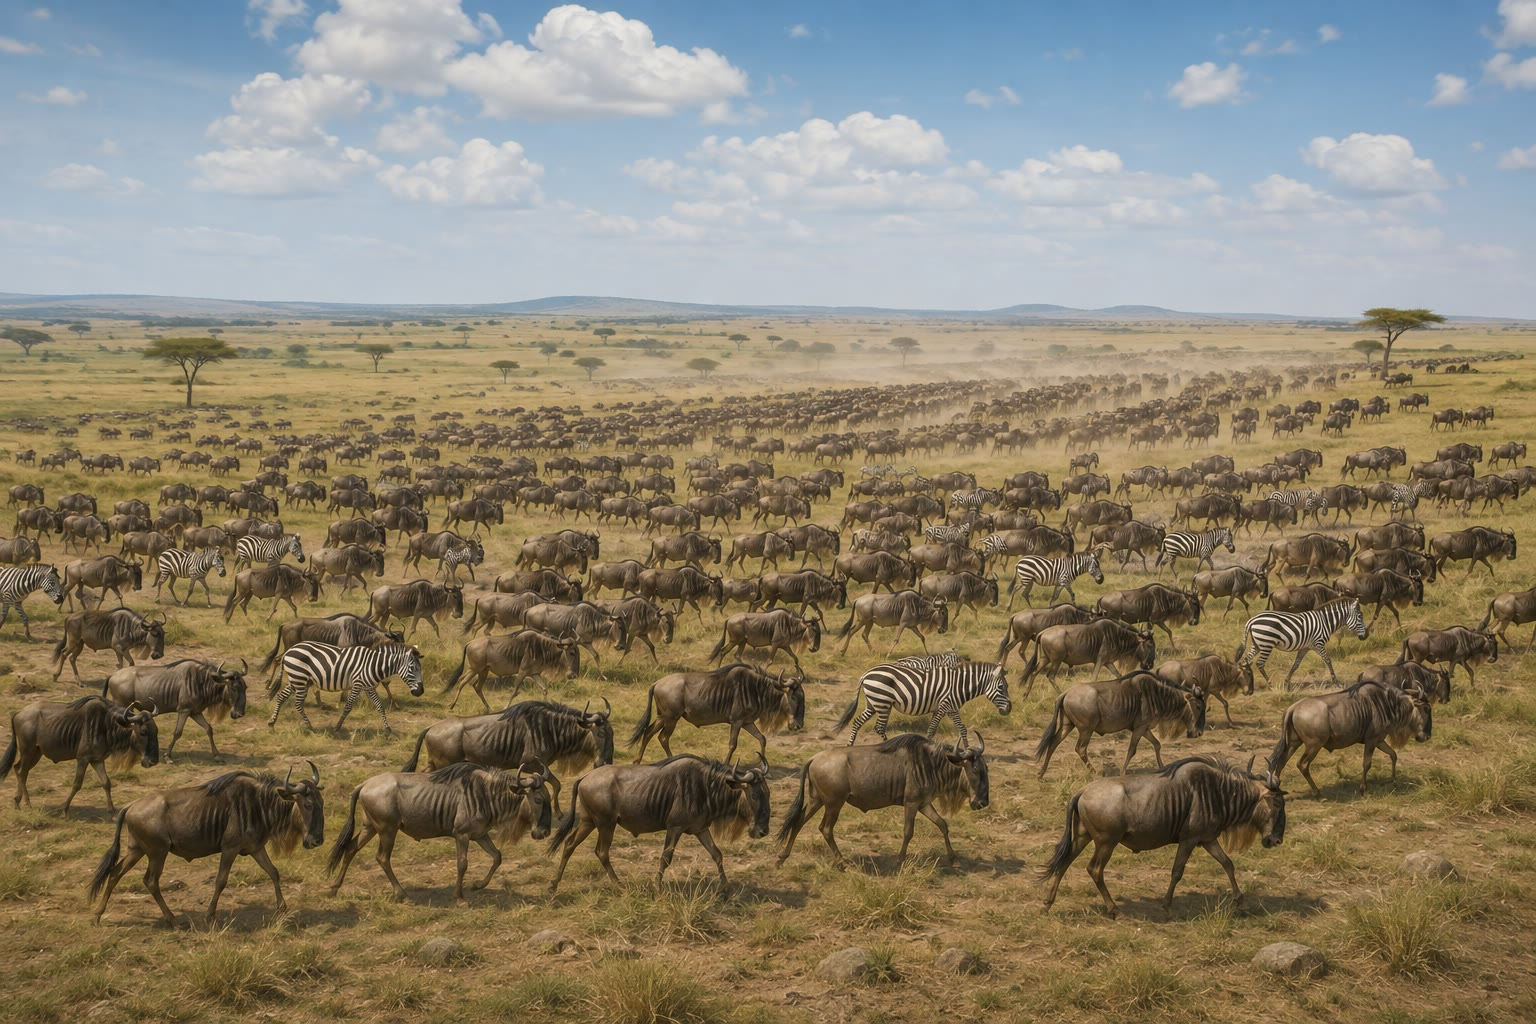
\includegraphics[width=0.6\linewidth]{images/book3/ai/b3-26-wildebeest-migration.jpg}

{\small 草原上的食草动物：由百万只动物组成的初级\omterm{def:b1:ecosystem-organization:trophic}{消费者}层级，
追随决定草地生产力的雨水迁徙，并
将其能量的十分之一传给身后的捕食者。}
\end{omfigure}

\section{统计多样性}

\begin{definition}[物种丰富度与多样性指数]\label{def:b1:ecosystem-organization:diversity}
\index{物种丰富度}\index{香农指数}
\omterm{def:b1:ecosystem-organization:ecosystem}{群落}的\emph{物种丰富度} $S$ 为其中物种的
数目。只看丰富度会忽略丰度：一片林地有一百棵栎树、
另外九种树各一棵，其多样性低于
每种各十棵的林地。\emph{香农指数}为
\[
H = -\sum_{i=1}^{S} p_i \ln p_i ,
\]
其中 $p_i$ 为属于物种 $i$ 的个体所占的比例，
随丰富度与\emph{均匀度}同时增大；
所有物种丰度相等时其值为 $\ln S$，某一物种占优时接近零。
\emph{均匀度}为 $H/\ln S$。一般而言，多样性由两极向热带增加，
随面积增大，随上次干扰后的时间延长，
并在一定程度内随地点生产力的提高而增加。
\end{definition}

\begin{method}[群落取样]\label{met:b1:ecosystem-organization:sampling}
\begin{enumerate}
  \item 根据生物选用合适的方法（样方、网具、
        陷阱、样线）取样，并记录每种
        生物的个体数。
  \item 以所发现的物种数对样本数
        （或个体数）作图：曲线先陡升，再
        趋于平缓；平缓处，丰富度已近完全。
        只有在取样强度相同时才可比较\omterm{def:b1:ecosystem-organization:ecosystem}{群落}。
  \item 计算 $H$ 与均匀度，并与等级–丰度图
        （物种按丰度排序，取对数刻度）比较，其
        斜率反映优势程度。
  \item 解释：均匀度低说明存在优势物种或
        胁迫；$H$ 随时间下降，说明
        \omterm{def:b1:ecosystem-organization:ecosystem}{生境}发生了变化。
\end{enumerate}
\end{method}

\begin{example}[两片林地]\label{ex:b1:ecosystem-organization:twowoods}
林地 A：100 棵栎树，另外九种树各一棵；$H = -(0.917\ln
0.917 + 9\times 0.0092\ln 0.0092) = 0.08 + 0.39 = 0.47$，均匀度
$0.47/2.30 = 0.20$。林地 B：同样十种树各十棵；$H =
\ln 10 = 2.30$，均匀度为 1。两者\omterm{def:b1:ecosystem-organization:diversity}{物种丰富度}相同，林地 B 的多样性是林地 A 的五倍。
\end{example}

\section{练习}

\begin{exercise}[$\star$]\label{exo:b1:ecosystem-organization:1}
给出\omterm{def:b1:ecosystem-organization:ecosystem}{生态系统}、\omterm{def:b1:ecosystem-organization:ecosystem}{群落}和\omterm{def:b1:ecosystem-organization:ecosystem}{生境}的定义，并以池塘为例说明。
\end{exercise}

\begin{exercise}[$\star$]\label{exo:b1:ecosystem-organization:2}
区分\omterm{def:b1:ecosystem-organization:niche}{栖息地}与\omterm{def:b1:ecosystem-organization:niche}{生态位}，并区分基础\omterm{def:b1:ecosystem-organization:niche}{生态位}与实际\omterm{def:b1:ecosystem-organization:niche}{生态位}。
\end{exercise}

\begin{exercise}[$\star$]\label{exo:b1:ecosystem-organization:3}
根据春季的能量金字塔，计算从
太阳光到总生产量的效率，以及净生产量中
被植食性动物取食的比例。
\end{exercise}

\begin{exercise}[$\star$]\label{exo:b1:ecosystem-organization:4}
说出四个营养类群，并指出
哪一类闭合了物质循环。
\end{exercise}

\begin{exercise}[$\star\star$]\label{exo:b1:ecosystem-organization:5}
某草地的\omterm{def:b1:ecosystem-organization:productivity}{净初级生产力}为 \qty{800}{g.m^{-2}.yr^{-1}}（\qty{17}{kJ/g}）。
兔子取食其中的 \qty{15}{\%}，同化所取食物的 \qty{50}{\%}，
并将所同化量的 \qty{5}{\%} 转化为兔子的生物量。计算
每公顷兔子的次级生产力，以及从\omterm{def:b1:ecosystem-organization:productivity}{净初级
生产力}到兔子的\omterm{thm:b1:ecosystem-organization:lindeman}{营养级效率}。
\end{exercise}

\begin{exercise}[$\star\star$]\label{exo:b1:ecosystem-organization:6}
解释为何生物量金字塔在海洋中可以倒置，而
能量金字塔则永不倒置。
\end{exercise}

\begin{exercise}[$\star\star$]\label{exo:b1:ecosystem-organization:7}
计算样本的\omterm{def:b1:ecosystem-organization:diversity}{香农指数}和均匀度，该样本中 A 有 50 个，B 有 30 个，C 有 15 个，
D 有 5 个。并与四个物种各 25 个的情形比较。
\end{exercise}

\begin{exercise}[$\star\star$]\label{exo:b1:ecosystem-organization:8}
在明暗瓶实验中，明瓶内的氧气
一天内增加 \qty{3}{mg/L}，暗瓶中的氧气则在一天内减少
\qty{1}{mg/L}。计算水体的\omterm{def:b1:ecosystem-organization:productivity}{总初级生产力}和\omterm{def:b1:ecosystem-organization:productivity}{净初级生产力}，
分别以每升每天的毫克氧气和克碳计。
（\qty{1}{g} $\mathrm{O_2}$ $\approx$ \qty{0.375}{g} C）。
\end{exercise}

\begin{exercise}[$\star\star$]\label{exo:b1:ecosystem-organization:9}
为何不存在十个环节的\omterm{def:b1:ecosystem-organization:foodweb}{食物链}，
岛屿和沙漠的\omterm{def:b1:ecosystem-organization:foodweb}{食物链}为何比森林的更短？
\end{exercise}

\begin{exercise}[$\star\star\star$]\label{exo:b1:ecosystem-organization:10}
人可以直接食用谷物，也可以用它来喂牛。
已知牛的\omterm{thm:b1:ecosystem-organization:lindeman}{营养级效率}为 \qty{10}{\%}，计算供养一人所需的土地面积，
分别按食用牛肉和直接食用谷物计，设农田每公顷产谷物
\qty{6}{t}，一人每年需要 \qty{1}{t}。
这说明了人类所处的\omterm{def:b1:ecosystem-organization:trophic}{营养级}，以及地球的
\omterm{thm:b1:populations:logistic}{环境容纳量}有何启示？
\end{exercise}

\begin{exercise}[$\star\star\star$]\label{exo:b1:ecosystem-organization:11}
开阔大洋每平方米的\omterm{def:b1:ecosystem-organization:productivity}{净初级生产力}很低，
却占全球生产量的一半。请调和二者，并解释为何海洋渔业
集中在其面积的百分之几之内。
\end{exercise}

\begin{exercise}[$\star\star\star$]\label{exo:b1:ecosystem-organization:12}
“\omterm{def:b1:ecosystem-organization:ecosystem}{生态系统}是把太阳光转化为热量的机器，生命只是
其副产品。”请用一段话讨论：能量流动与物质循环的对比，
\omterm{def:b1:ecosystem-organization:trophic}{分解者}的作用，以及这句话遗漏了什么。
\end{exercise}

\section{问题：泉的能量收支}

\begin{problem}[{周末问题——奥德姆的泉按营养级逐级展开：
由阳光到草、草到蜗牛、蜗牛到鱼、鱼到
苍鹭，并包括呼吸作用与分解者，
最后给出各营养级的效率}]
\label{pb:b1:ecosystem-organization:1}
泉每年每平方米接收 \qty{1.7e6}{kcal} 的阳光。
其\omterm{def:b1:ecosystem-organization:trophic}{生产者}固定 \qty{20800}{kcal}（总量），并呼吸消耗
\qty{12000}{}。植食性动物取食 \qty{3400}{kcal} 植物物质，
其中同化 \qty{1500}{}，呼吸消耗 \qty{1100}{}，其余
转化为生长和后代。食肉动物取食 \qty{380}{kcal}，呼吸消耗
\qty{300}{}，其余则用于生产；顶级食肉动物取食 \qty{20}{kcal}，
呼吸消耗 \qty{14}{}，生产 \qty{6}{}。未被取食或呼吸的部分
均流向\omterm{def:b1:ecosystem-organization:trophic}{分解者}，并由其呼吸消耗。取
\qty{1}{kcal} $= \qty{4.18}{kJ}$，且每克
干生物量含 \qty{10}{kcal}。

\medskip
\noindent\textbf{第一部分——\omterm{def:b1:ecosystem-organization:trophic}{生产者}。}
\begin{enumerate}
  \item 计算\omterm{def:b1:ecosystem-organization:productivity}{净初级生产力}。
  \item 计算光合作用效率，即总生产量
        与阳光之比。将其与
        在\cref{ch:b1:photosynthesis}中的 \qty{34}{\%} 相比较，并列出
        导致二者差异的三种损失。
  \item \omterm{def:b1:ecosystem-organization:trophic}{生产者}呼吸消耗的量占总生产量
        的比例为多少？
  \item 净生产量中有多少被植食性动物取食，
        有多少直接进入\omterm{def:b1:ecosystem-organization:trophic}{分解者}？
  \item 将\omterm{def:b1:ecosystem-organization:productivity}{净初级生产力}换算为每平方米每年的克干物质，
        并将该泉置于本章所述的生物群系之中。
  \item 每平方米每年，有多少阳光以热量形式
        离开该泉，而从未经过任何活的
        \omterm{def:b1:organism-environment:organism}{生物体}？
\end{enumerate}

\medskip
\noindent\textbf{第二部分——\omterm{def:b1:ecosystem-organization:trophic}{消费者}。}
\begin{enumerate}[resume]
  \item 计算植食性动物的次级生产力，以及其
        同化效率（同化量/取食量）。
  \item 计算植食性动物的生产效率
        （生产量/同化量）。
  \item 计算从\omterm{def:b1:ecosystem-organization:trophic}{生产者}到植食性动物的\omterm{thm:b1:ecosystem-organization:lindeman}{营养级效率}：
        植食性动物的生产量与\omterm{def:b1:ecosystem-organization:productivity}{净初级生产力}之比。
  \item 计算食肉动物的生产量，以及从植食性动物
        到食肉动物的\omterm{thm:b1:ecosystem-organization:lindeman}{营养级效率}。
  \item 计算从食肉动物到顶级食肉动物的\omterm{thm:b1:ecosystem-organization:lindeman}{营养级效率}。
  \item 每平方米每年有多少能量到达顶级食肉动物
        的自身\omterm{def:b1:body-plans-tissues:tissue}{组织}？这部分占阳光的
        比例是多少？
  \item 为何同化效率从植食性动物到
        食肉动物逐级升高？
\end{enumerate}

\medskip
\noindent\textbf{第三部分——\omterm{def:b1:ecosystem-organization:trophic}{分解者}与平衡。}
\begin{enumerate}[resume]
  \item 列出流向\omterm{def:b1:ecosystem-organization:trophic}{分解者}的各项（未被取食的净生产量、
        植食性动物粪便及未被取食的植食性动物生产量等），
        并将它们求和。
  \item 计算该\omterm{def:b1:ecosystem-organization:ecosystem}{生态系统}的总呼吸量：\omterm{def:b1:ecosystem-organization:trophic}{生产者}、
        植食性动物、食肉动物、顶级食肉动物和\omterm{def:b1:ecosystem-organization:trophic}{分解者}。
  \item 将其与总初级生产量比较。该比较结果对
        一年内春季水体的生物量意味着什么？
  \item 被\omterm{def:b1:ecosystem-organization:trophic}{分解者}呼吸消耗的部分占总初级生产量的
        比例是多少？
  \item 画出能量金字塔，标出四个\omterm{def:b1:ecosystem-organization:trophic}{营养级}的生产量，
        并标注各效率值。
\end{enumerate}

\medskip
\noindent\textbf{第四部分——存量、周转与变化。}
各\omterm{def:b1:ecosystem-organization:trophic}{营养级}的现存生物量分别为：\omterm{def:b1:ecosystem-organization:trophic}{生产者} \qty{800}{g/m^2}，植食性动物 \qty{40}{g/m^2}，
食肉动物 \qty{10}{g/m^2}，顶级
食肉动物 \qty{1.5}{g/m^2}。
\begin{enumerate}[resume]
  \item 将各级生物量换算为千卡，并画出生物量
        金字塔。它是正立的吗？
  \item 计算各\omterm{def:b1:ecosystem-organization:trophic}{营养级}的周转时间（生物量/生产量）。
        哪一级周转最快？原因是什么？
  \item 一只重 \qty{2}{kg} 的鹭以春季水体的顶级食肉动物的
        生产量为食。它需要多少平方米的面积？
  \item 春季水体施加肥料后，其总初级生产量
        翻倍，但植食性动物的取食速度无法加快。
        额外的生产量、\omterm{def:b1:ecosystem-organization:trophic}{分解者}的呼吸量
        以及夜间水中的氧气会发生什么变化？
  \item 引入一种新的鱼类，它取食植食性动物的卵，
        并使植食性动物的生产量减半。预测食肉动物的生产量、
        鹭的数量以及鳗草的命运。
  \item 解释为何移除顶级食肉动物对鳗草的影响
        远大于移除等量能量所对应的
        植食性动物。
  \item 给出结果：三次转移各自的\omterm{thm:b1:ecosystem-organization:lindeman}{营养级效率}、
        阳光到总初级生产量的效率，以及
        太阳能中到达
        顶级食肉动物的比例。
\end{enumerate}
\end{problem}
